% Chapter 2: Background

% Length: aim for 10-15 pages

This chapter presents the different background topics of the thesis work, which are the long-tailed datasets, model architectures \textit{Convolutional Neural Networks (CNN)} and \textit{Vision Transformers (VT)}, the deep long-tailed learning methods \textit{Class Re-balancing (CR)}, \textit{Information Augmentation (IA)}, 
and \textit{Module Improvement (MI)}. These topics will be explained for the reader.

\todo{Mention image classification, as it is the primary goal of this thesis.} 

% ===============================================================================
% LT Datasets

\section{Long-Tailed Datasets}
\label{sec:lt-datasets}
Long-tailed datasets pose significant challenges in deep learning, as they represent an extreme form of class imbalance. Addressing these challenges is central to this thesis, which explores methods to improve model performance on underrepresented classes. This section outlines the structure of long-tailed distributions and their implications.

A balanced dataset is one where all classes are evenly represented, whereas imbalanced datasets feature varying sample sizes across classes. Long-tailed datasets are characterized by a significant class imbalance, where a few dominant classes account for most samples (head classes), while the majority of classes are underrepresented (tail classes) as depicted in Figure \ref{fig:lt_distribution}. This  distribution is common for real-world datasets \cite{Newman_2005, liu2019largescalelongtailedrecognitionopen}. For example, the iNaturalist, a popular benchmark for image classification, exhibits a long-tailed distribution of species \cite{vanhorn2018inaturalistspeciesclassificationdetection}. Other benchmarks are constructed by sampling from datasets such as ImageNet \cite{ImageNet2009} by using a Pareto distribution, which simulates long-tailed class distributions with a power-law decay \cite{zhang2023deep, dealvis2024surveydeeplongtailclassification,cao2019learningimbalanceddatasetslabeldistributionaware}.

CIFAR100-LT \cite{cao2019learningimbalanceddatasetslabeldistributionaware}, derived from the CIFAR-100 dataset \cite{krizhevsky2009learning}, serves as the primary dataset for the experiments conducted in this thesis. CIFAR-100 is a widely used benchmark in classification research due to its diverse class representation and manageable size. It consists of 60,000 32x32 color images divided into 100 classes, each with 600 samples. These are further split into 500 training images and 100 testing images per class. CIFAR100-LT is created by reducing the number of samples in certain classes of CIFAR-100 following an exponential decay en sample sizes, given by:

\begin{equation}
    \label{eq:exp}
    n_i = n_{max}\cdot \text{IR}^{\frac{i-1}{C-1}}
\end{equation}

Where $n_i$ is the number of samples in class $i$, $n_{max}$ is the number of samples in the most frequent class, IR is the imbalance ratio, and $C$ is the total number of classes \cite{kaidic_ldam_drw}.

Other long-tailed datasets follow a Pareto distribution with number of samplers per class as followed \cite{liu2019largescalelongtailedrecognitionopen}:

\begin{equation}
    \label{eq:pareto}
    f(C) = \frac{\alpha C_{\text{m}}^\alpha}{C^{\alpha + 1}}, \quad C \geq C_{\text{m}}, \quad \alpha > 0
\end{equation}

Here, $\alpha$ is the shape parameter, $C_{\text{m}}$ is the scale parameter representing the minimum possible class index, and $C$ is the class index. A larger $\alpha$ results in a more severe imbalance.

    


\begin{figure}[ht]
    \centering
    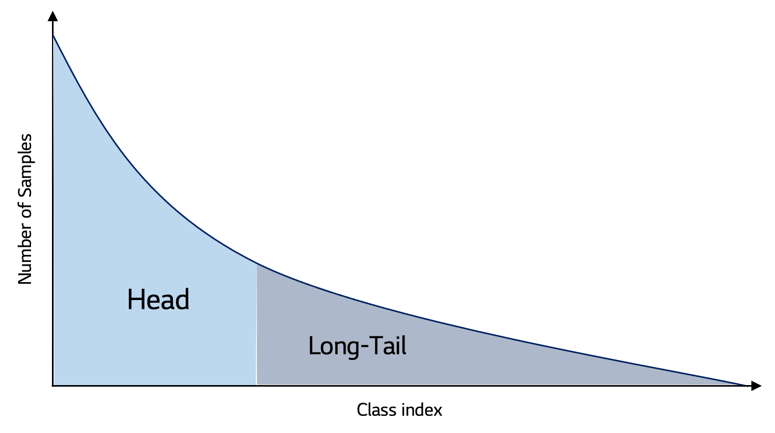
\includegraphics[width=0.8\textwidth]{Images/long_tail_distribution.png} 
    \caption{Illustration of a long-tailed distribution. Figure from \cite{lgresearch257}.}
    \label{fig:lt_distribution} % Use a unique label for referencing the figure
\end{figure}

Class imbalance has a profound impact on model performance compared to evenly distributed datasets \cite{vanhorn2017deviltailsfinegrainedclassification, cui2019classbalancedlossbasedeffective}. Deep networks trained on long-tailed datasets often exhibit biased performance, favoring head classes while performing poorly on tail classes \cite{zhang2023deep}. Zhang et al. (2023) provide a comprehensive survey of methods addressing this challenge, categorizing current approaches into three main groups: class re-balancing, information augmentation, and module improvement. These methods will be further explored in section \ref{sec:lt_methods}. 


% ===============================================================================
% Model architechtures

\section{Model Architecures}
\label{sec:model_arch}
Deep learning has revolutionized image classification by introducing models capable of learning complex patterns and representations from data. Among these, Convolutional Neural Networks (CNNs) and Vision Transformers (ViTs) are chosen as the primary architectures used in this thesis due to their performance on image classification tasks. This section provides a theoretical foundation for these models, focusing on the specific architectures utilized: MobileNetV2 \cite{sandler2018mobilenetv2}, ResNet50V2 \cite{he2016}, and ConvNeXt Base \cite{todi2023convnext} as the CNN architectures, and ViT-B/16 \cite{dosovitskiy2021imageworth16x16words} as the ViT architecture.

\todo{A brief summary of the relevance of the chosen architectures so that the reader knows why they are included.}

% ===============================================================================
% DNNs

\subsection{Introduction to Deep Neural Networks}
\label{sec:intro_DNN}
Before the introduction of Convolutional Neural Networks (CNNs) and, more recently, Vision Transformers (ViTs), the standard approach for image classification involved flattening a two-dimensional image matrix into a one-dimensional array and passing it through a Multilayer Perceptron (MLP), also known as a feed-forward neural network. MLPs are fully connected neural networks composed of an input layer, output layer, and one or more hidden layers. Being fully connected means that each neuron in a given layer is connected to all neurons in the next layer, forming a dense network. These connections are associated with weights and biases, which the network learns during training. Input features are fed into the input layer, propagated through hidden layers that add complexity to model nonlinear relationships, and yield predictions in the output layer. Known as universal approximators, MLPs can approximate any continuous function given sufficient neurons in the hidden layers \cite{zhang2023dive,HORNIK1989359}.

To illustrate the structure of a neural network, figure \ref{fig:dnn_layers} shows an example of a feed-forward neural network with three input neurons, two hidden layers, each with four neurons, and two output neurons. This architecture could be used, for instance, to classify images of cats and dogs based on three input features, such as height, weight, and width of the animals. The input propagates through the network, with each neuron computing a weighted sum of its inputs followed by an optional nonlinearity. The final output is a prediction, where the class corresponding to the neuron with the highest value is chosen.

\begin{figure}[ht]
    \centering
    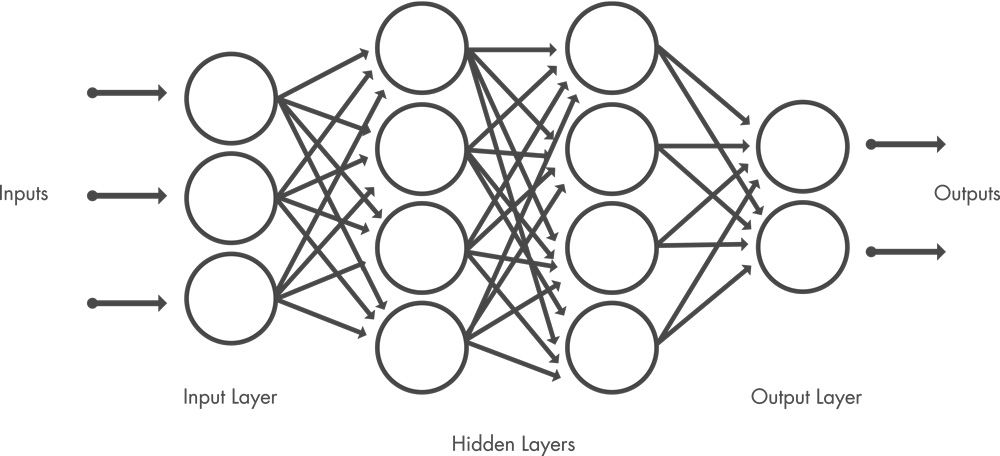
\includegraphics[width=0.8\textwidth]{Images/cnn_layers.jpg} 
    \caption{Layers of a neural network. Figure from \cite{mathworks_cnn}. \todo{Make this figure.}}
    \label{fig:dnn_layers}
\end{figure}

However, this simple neural network becomes insufficient for more complex problems, such as image classification, as it requires an increasing number of parameters. For instance, a $224\times 224$ RGB image flattened is very large, making MLPs parameter-heavy and inefficient. The limitations of MLPs were addressed by Convolutional Neural Networks (CNNs), which introduced convolutional and pooling layers to effectively preserve and utilize the spatial information of pixels in two-dimensional images \cite{zhang2023dive}.

% ===============================================================================
% CNNs

\subsection{Convolutional Neural Networks}
\label{sec:CNNs}
\todo{finish this section.}

% What are CNNs?
% Historical context.
% Input data.
% Output data.
% Layers.

% Before the CNNS, the standard was to flatten the image from two dimensional matrix into a one dimensional array and pass it through a feed-forward neural network in order to classify the image. As the image is converted into one dimension, naturally, spacial information in the image is lost. 

% As is common for all neural networks, they are made up of neurons with learnable weights and biases, and has an input layer and an output layer with several hidden layers in between, where each hidden layer can have an arbitrary amount of neurons. Each neron recieves some inputs, perfom dot product and optionally follows it with nonlinearity.

%  A simple neural network is illustrated in figure \ref{fig:cnn_layers}, which shows an NN with three input neurons, two hidden layers with four neurons each, and an output layer of two neurons. The example in figure \ref{fig:cnn_layers} could be a neural network designed to classify cats and dogs based on three parameters. The parameters could be height, weight, and nose length of the pet. This data would propagate through the NN and the result would be the value of the two output neurons. The output with the highest value would be intrepreted as the class of the given input data, either a cat or a dog. The idea is that a neural network functions as a universal approximator, and without the hidden layers, it is just a linear function \cite{zhang2023dive}. The hidden layers introduce nonlinearity  
 

Convolutional Neural Networks (CNNs) \cite{lecun1995} were introduced to address the limitations of MLPs for image-related tasks. Unlike MLPs, which treat input features as independent, CNNs are designed to recognize patterns in images by applying local filters through convolutional layers, and thereby preserving the two dimensional input of an image, preserving the idea that nearby pixels are related \cite{lecun1998,NIPS2012_c399862d,zhang2023dive}. %CNNs exploit the spatial structure of images by applying local filters through convolutional layers. This approach preserves important relationships between neighboring pixels and enables more efficient learning of visual patterns \cite{lecun1998,NIPS2012_c399862d}.


CNNs consist of several core components, as illustrated in Figure~\ref{fig:cnn_illustration}. They have three main layers: convolutional layers, pooling layers, and a fully connected layer. The convolutional layer is the first layer, and serves to extract local features by applying filters to small regions of an image, while pooling layers reduce the spatial dimensions of feature maps, providing invariance to small translations. The CNN can be made up of multiple convolution and pooling layers, but the fully connected layer will be the final layer. Activation functions introduce nonlinearity, allowing the network to capture complex patterns. At the final stage, fully connected or global pooling layers aggregate the extracted features into predictions, enabling tasks such as classification or segmentation.


\begin{figure}[ht]
    \centering
    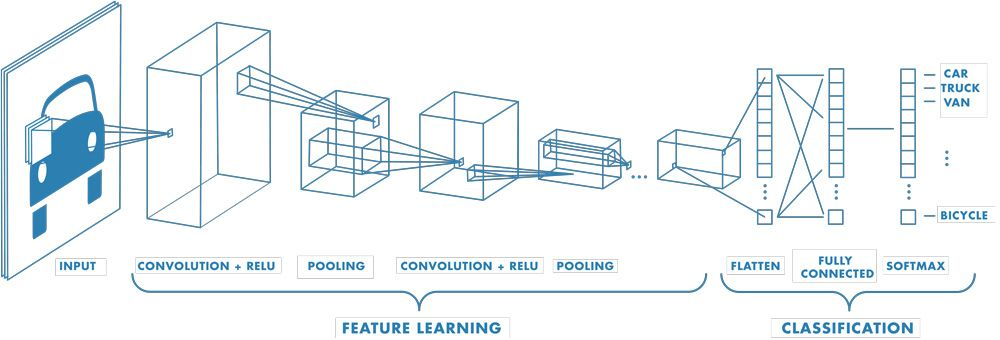
\includegraphics[width=0.8\textwidth]{Images/CNN_illustration.jpg} 
    \caption{Illustration of a convolutional neural network. Figure from \cite{mathworks_cnn}. \todo{Make this figure.}}
    \label{fig:cnn_illustration}
\end{figure}

\todo{Tie to the models used for experiments in this thesis.}
\url{https://www.ibm.com/topics/convolutional-neural-networks}

CNNs gained popularity after the introduction of LeNet-5 by LeCun et al. in 1998 \cite{lecun1998} that demonstrated the potential of CNNs by recognizing handwritten digits. Later, AlexNet \cite{NIPS2012_c399862d} achieved a breakthrough by winning the ImageNet Challenge in 2012, demonstrating the potential of CNNs to handle large-scale image recognition tasks by deepening the architechtures and utilizing multiple GPUs for training. Subsequently, the evolution of CNNs has progressed through architectures such as VGGNet \cite{simonyan2015deepconvolutionalnetworkslargescale}, GoogLeNet \cite{szegedy2014goingdeeperconvolutions}, and ResNet \cite{he2016}, which have set the stage for the advancements seen in modern CNNs.

% ===============================================================================
% ResNet50

\subsubsection{ResNet50 Architecture}
\label{sec:resnet}
\todo{write this section.}
ResNet50 is a variant of the ResNet (Residual Network) architecture, which introduced the concept of residual learning to address the vanishing gradient problem in deep networks \cite{he2016}. 



% ===============================================================================
% MobileNetV2

\subsubsection{MobileNetV2 Architecture}
\label{sec:mobilenet}
MobileNetV2 introduced by Sandler et al. \cite{sandler2018mobilenetv2} is a lightweight CNN model designed primarily to balance model accuracy and computational efficiency, making it suitable for mobile or embedded devices. Building upon the original concepts of MobileNetV1 \cite{howard2017mobilenetsefficientconvolutionalneural}, MobileNetV2 preserves the use of depthwise separable convolutions, a method for reducing the parameters and floating-point operations, while introducing a novel element known as the inverted residual structure. 

% \begin{figure}[ht]
%     \centering
%     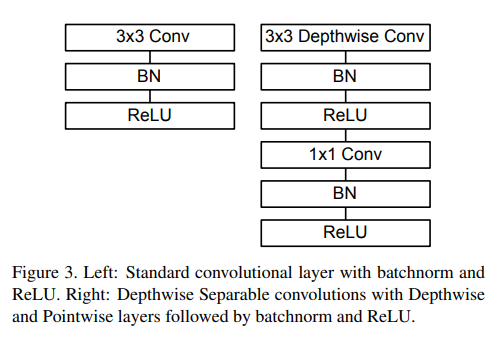
\includegraphics[width=0.8\textwidth]{Images/mobilenet_structure.png} 
%     \caption{Illustration of the MobileNetV1 structure. Figure from \cite{howard2017mobilenetsefficientconvolutionalneural}. \todo{Make this figure.}}
%     \label{fig:MobileNetV1_structure}
% \end{figure}

\paragraph{Inverted Residual Blocks}
While traditional residual connections, introduced in Residual Networks (ResNets) \cite{he2016} \todo{as discussed in the previous section}, allow for identity mapping and improved gradient flow, MobileNetV2 employs an inverted residual structure \cite{sandler2018mobilenetv2}. Instead of mapping from a high-dimensional representation down to a lower-dimensional bottleneck, then reconstructing features at the output, inverted residual blocks begin with a low-dimensional input and expand it to a higher-dimensional space before applying a depthwise convolution. After spatial filtering, the representation is projected back down to a low-dimensional space. This approach, illustrated in Figure \ref{fig:residual}, helps preserve crucial information and maintain a rich feature space without substantially increasing computational cost. The use of a linear bottleneck (i.e., no nonlinear activation in the low-dimensional projection) also helps prevent the destruction of useful information, further improving efficiency and accuracy.  

\begin{figure}[ht]
    \centering
    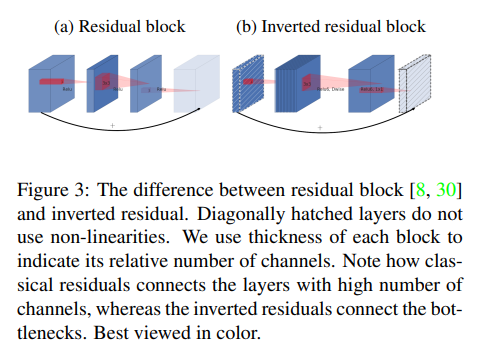
\includegraphics[width=0.8\textwidth]{Images/inverted_residual.png} 
    \caption{Residual and Inverted Residual Blocks. Figure from \cite{sandler2018mobilenetv2}. \todo{Make this figure.}}
    \label{fig:residual}
\end{figure}

\paragraph{Depthwise Separable Convolution}
Following MobileNetV1, MobileNetV2 relies on depthwise separable convolutions to factorize the convolution operation into two simpler operations \cite{howard2017mobilenetsefficientconvolutionalneural}: depthwise convolution and pointwise convolution as shown in figure \ref{fig:depthwise_sep_conv}. The depthwise convolution applies a single filter to each input channel, and the pointwise convolution (a $1\times 1$ convolution) then recombines the channels to produce the desired output. In comparison, a standard convolution both filtes and combines inputs into a new set of outputs. This approach reduces the parameter count and computational load, making the model suitable for devices with limited resources \cite{howard2017mobilenetsefficientconvolutionalneural,sandler2018mobilenetv2}.

\begin{figure}[ht]
    \centering
    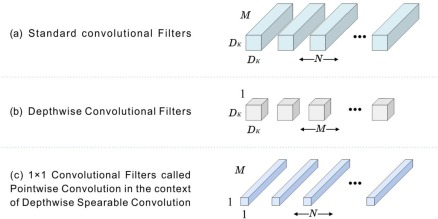
\includegraphics[width=0.8\textwidth]{Images/depthwise_separable_conv.jpg} 
    \caption{Depthwise Separable Convolution. Figure from \url{https://www.sciencedirect.com/topics/computer-science/depthwise-separable-convolution}. \todo{Make this figure.}}
    \label{fig:depthwise_sep_conv}
\end{figure}


\paragraph{Relevance}
In this thesis, MobileNetV2 represents an example of a modern, efficient CNN architecture. Its lightweight design makes it particularly attractive for applications where computational resources are limited. By including MobileNetV2 among the evaluated architectures, the performance is compared across varying complexity levels, providing insights into how efficiency-oriented designs fare against more complex models. This comparison is especially relevant if the application domain involves real-time processing or deployment on mobile or embedded devices.

% "This lightweight MobileNetV2 CNN model was proposed by Sandler et al. [24] in 2019. It is based on the MobileNetV1 architecture given by Howard et al. [25] in 2017. MobileNetV2 is a 53-layer deep lightweight CNN model with fewer parameters and an input size of 224x224. The MobileNetV1 architecture used the concept of depth-wise separable convolutions that applies a single filter to each input channel, and the point-wise convolutions (1x11x1) aim at combining the output of the depth-wise convolutions. The MobileNetV2 lightweight CNN model is made up of mainly two blocks: (a) block with stride=[1 1], often called the residual block with S=[1 1]; and (b) block with stride=[2 2], which mainly aims at downsizing. The depth-wise convolution performs filtering, which is lightweight in nature. This is achieved simply by applying one convolution filter per input channel and forms the first layer of the MobileNetV2 blocks. The 1x1 convolution forms the second layer of the MobileNetV2 blocks and is known as the point-wise convolution. These 1x1 convolutions are responsible for structuring new features through the linear combination of input channels. Fig. 7.5 shows the structure of the building blocks of the MobileNetV2 CNN model with stride=[1 1] and stride=[2 2]. The MobileNetV2 CNN model has been widely used in medical image analysis [20, 26-34]" \url{https://www.sciencedirect.com/topics/computer-science/mobilenetv2}



% ===============================================================================
% ConvNeXt Base

\subsubsection{ConvNeXt Base Architecture}
\label{sec:convnext}
\todo{Write this section.}
ConvNeXt Base is a modernized CNN architecture inspired by insights from transformer-based models, designed to achieve competitive performance while retaining the efficiency of CNNs \cite{todi2023convnext}. Notable features include:

Simplified Design: Incorporates architectural refinements such as depthwise convolutions and LayerNorm.
Enhanced Efficiency: Balances accuracy and computational cost, bridging the gap between traditional CNNs and transformer-based models. 

Improvement from predecessors: integrating insights from ViTs.

"The "Roaring 20s" of visual recognition began with the introduction of Vision Transformers (ViTs), which quickly superseded ConvNets as the state-of-the-art image classification model. A vanilla ViT, on the other hand, faces difficulties when applied to general computer vision tasks such as object detection and semantic segmentation. It is the hierarchical Transformers (e.g., Swin Transformers) that reintroduced several ConvNet priors, making Transformers practically viable as a generic vision backbone and demonstrating remarkable performance on a wide variety of vision tasks. However, the effectiveness of such hybrid approaches is still largely credited to the intrinsic superiority of Transformers, rather than the inherent inductive biases of convolutions. In this work, we reexamine the design spaces and test the limits of what a pure ConvNet can achieve. We gradually "modernize" a standard ResNet toward the design of a vision Transformer, and discover several key components that contribute to the performance difference along the way. The outcome of this exploration is a family of pure ConvNet models dubbed ConvNeXt. Constructed entirely from standard ConvNet modules, ConvNeXts compete favorably with Transformers in terms of accuracy and scalability, achieving 87.8 \% ImageNet top-1 accuracy and outperforming Swin Transformers on COCO detection and ADE20K segmentation, while maintaining the simplicity and efficiency of standard ConvNets." \url{https://paperswithcode.com/paper/a-convnet-for-the-2020s}

% ===============================================================================
% Vision Transformers

\subsection{Vision Transformers}
\label{sec:ViTs}
\todo{Explain their advantages over CNNs for certain tasks.
Mention why they are relevant for handling long-tailed datasets.}

% ===============================================================================
% ViT-B/16

\subsubsection{ViT-B/16 Architecture}
\label{sec:vitb16}
\todo{write this section.}
ViT-B/16 is a Vision Transformer model that leverages the transformer architecture for image classification \cite{dosovitskiy2021imageworth16x16words}. Key characteristics include:

Patch Embeddings: Images are divided into 16x16 patches, which are then flattened and embedded.
\url{https://sh-tsang.medium.com/review-vision-transformer-vit-406568603de0}

The Vision Transformer, or ViT, is a model for image classification that employs a Transformer-like architecture over patches of the image. An image is split into fixed-size patches, each of them are then linearly embedded, position embeddings are added, and the resulting sequence of vectors is fed to a standard Transformer encoder. In order to perform classification, the standard approach of adding an extra learnable “classification token” to the sequence is used.
\url{https://paperswithcode.com/method/vision-transformer}

%====================================================================================

\section{Classic Long-Tailed Methods}
\label{sec:lt_methods}
\todo{Introduce the three methods (CR, IA, MI) with a brief explanation of their purpose.}

Following the paper \textit{Deep Long-Tailed Learning: A Survey} \cite{zhang2023deep}, the existing deep long-tailed learning methods are grouped into three main categories based on their technical approach: class re-balancing, information augmentation, and module improvement. These categories are further divided onto sub-categories: re-sampling, class-sensitive learning, logit adjustment, transfer learning, data augmentation, representation learning, classifier desing, decoupled training, and ensemble learning as shown on figure \ref{fig:lt_main_categories}. This thesis does not aim to examine all the beforementioned method, but aims to find a deep learning approach to a specific problem. The backgrounds of the methods used in this thesis are described in this section.

\begin{figure}[ht]
    \centering
    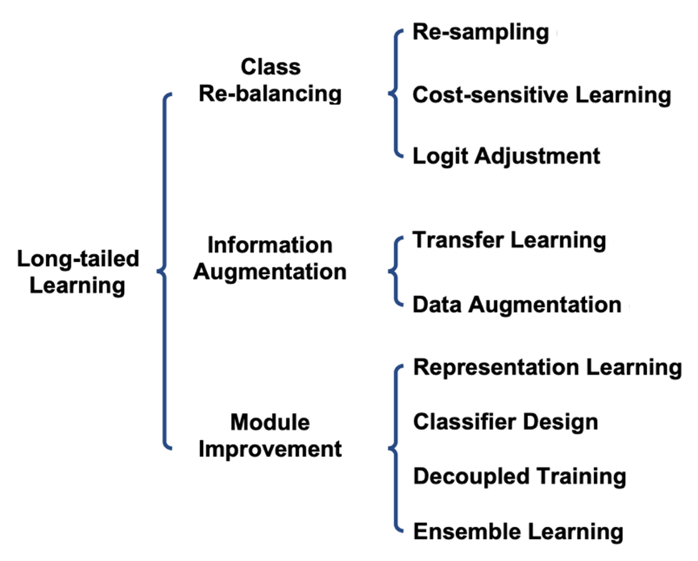
\includegraphics[width=0.8\textwidth]{Images/lt_methods_categories.png} 
    \caption{Long-tailed categories as described by \textit{Zhang et al.} \cite{zhang2023deep}.}
    \label{fig:lt_main_categories} % Use a unique label for referencing the figure
\end{figure}

\subsection{Class Re-balancing}
The class re-balancing method aims to re-balance the effect of the imbalanced training dataset, and has three main sub-categories: re-sampling, class-sensitive learning, and logit adjustment \cite{zhang2023deep}. 

\subsubsection{Re-sampling}
The traditional way to sample when training deep networks is using mini-batch gradient descent with random sampling. This means that each sample has an equal probability of being sampled. When sampling from an imbalanced dataset, samples from head classes naturally occur more often, and thus have higher chance of being sampled than samples from tail classes, making the resulting deep models biased towards head classes. Re-sampling is a method that adresses this problem by adjusting the number of samples per class in each sample batch for model training. 

\subsubsection{Class-sensitive Learning}
% The loss function serves as a measure of the model's fitness to the data, quantifying the distance between the actual and predicted values of the target. Typically, the loss is represented as a nonnegative value, where smaller values indicate a better fit, and a perfect fit corresponds to a loss of zero \cite{zhang2023dive}. 

% Conventional training of deep networks using the softmax cross-entropy loss often overlooks class imbalance. This results in uneven gradients for different classes, leading to suboptimal performance on underrepresented classes. To mitigate this issue, modifications to the loss function are introduced to ensure a more balanced contribution from each class during training.

Traditional training methods using the standard loss function, cross-entropy loss, can lead the model to be biased towards head classes, as the loss ignores class imbalance and thus generate an uneven amount of gradients for different classes \cite{zhang2023deep}. Consequently, tail classes are often misclassified. To address this imbalance, class-sensitive learning methods modify the loss function to pay more attention to minority classes, thus improving overall performance.

Two prominent categories of class-sensitive strategies are \emph{re-weighting} and \emph{re-margining}. Re-weighting involves adjusting the contribution of each class to the loss by multiplying them with different weights. By carefully selecting these weights, the model allocates a higher penalty to misclassification of underrepresented classes, thus re-balancing the training process \cite{zhang2023deep}. Re-margining, on the other hand, modifies the decision boundaries by introducing class-dependent margins, ensuring that minority classes have more room to establish discriminative features in the embedding space \cite{zhang2023deep, cao2019learningimbalanceddatasetslabeldistributionaware}.

In what follows, the theory behind several representative loss functions commonly used in class-sensitive learning is presented, beginning with the baseline Softmax Cross-Entropy loss. Subsequently, the theory behind multiple re-weighting schemes including Weighted Softmax Cross-Entropy, Focal Loss, Class-Balanced Loss, Balanced Softmax Loss, and Equalization Loss, as well as a re-margining method exemplified by LDAM Loss. Each of these methods seeks to improve the imbalance in training through modifications that ultimately improve the classification performance on tail classes.


% \subsubsection{Loss Functions for Class-Sensitive Learning}
% The loss function serves as a measure of the model's fitness to the data, quantifying the distance between the actual and predicted values of the target. 
Table \ref{tab:loss_summary} summarizes the loss functions employed for class-sensitive learning used in this thesis, outlining their formulations and categorizations into re-weighting or re-margining strategies.


\begin{table}[H]
    \centering
    \caption{Summary of losses.}
    \label{tab:loss_summary}
    \begin{tabular}{|l|l|c|}
    \hline
    \textbf{Loss Name}       & \textbf{Formulation}                                                & \textbf{Type}        \\ \hline
    Softmax loss \cite{pytorch_crossentropy}             & $L_{ce} = - \log(p_y)$                                              & -                   \\
    Focal loss \cite{lin2018focallossdenseobject}     & $L_{fl} = -(1 - p_y)^\gamma \log(p_y)$                             & re-weighting        \\
    Weighted Softmax loss \cite{zhang2023deep}    & $L_{wce} = - \frac{1}{\pi_y} \log(p_y)$                           & re-weighting        \\
    Class-balanced loss \cite{cui2019classbalancedlossbasedeffective} & $L_{cb} = - \frac{1 - \gamma}{1 - \gamma^{n_y}} \log(p_y)$         & re-weighting        \\
    Balanced Softmax loss \cite{ren2020balancedmetasoftmaxlongtailedvisual} & $L_{bs} = - \log\left( \frac{\pi_y \exp(z_y)}{\sum_j \pi_j \exp(z_j)} \right)$ & re-weighting        \\
    Equalization loss \cite{tan2020equalizationlosslongtailedobject} & $L_{eq} = - \log\left( \frac{\exp(z_y)}{\sum_j \omega_j \exp(z_j)} \right)$    & re-weighting        \\
    LDAM loss \cite{cao2019learningimbalanceddatasetslabeldistributionaware}      & $L_{ldam} = - \log\left( \frac{\exp(z_y - \Delta_y)}{\sum_j \exp(z_j - \Delta_j)} \right)$ & re-margining        \\
    \hline
    \end{tabular}
    \end{table}

% From \cite{zhang2023deep}: Conventional training of deep networks is based on the softmax
% cross-entropy loss (c.f. Table 3). This loss ignores the class
% imbalance in data sizes and tends to generate uneven gradients for
% different classes. That is, each positive sample of one class can be
% seen as a negative sample for other classes in cross-entropy, which
% leads head classes to receive more supporting gradients (as they
% usually are positive samples) and causes tail classes to receive more
% suppressed gradients (as they usually are negative samples) [19],
% [55]. To address this, class-sensitive learning seeks to particularly
% adjust the training loss values for various classes to re-balance
% the uneven training effects caused by the imbalance issue [132],
% [133], [134], [135], [136], [137]. There are two main types of
% class-sensitive strategies, i.e., re-weighting and re-margining. We
% begin with class re-weighting as follows.

\paragraph{Softmax Cross-Entropy Loss}

The \emph{Softmax Cross-Entropy (CE) loss} is a fundamental building block in training deep classifiers and is widely regarded as the baseline in classification tasks \cite{zhang2023deep, cs231n, pytorch_crossentropy}. 

The \textit{Softmax} function transforms the raw output scores (logits) of the final layer of a neural network into a probability distribution over \( K \) classes. For an input \( \mathbf{z} = [z_1, z_2, \dots, z_K] \), the Softmax function for class \( i \) is defined as:

\begin{equation}
    P(y = i \mid \mathbf{z}) = \frac{\exp(z_i)}{\sum_{j=1}^{K} \exp(z_j)}
\end{equation}

Here, \( \exp(z_i) \) ensures that all values are positive, and dividing by the sum normalizes the probabilities so that they sum to 1. This normalization is crucial for classification, as it allows the network's outputs to represent the likelihood of each class.

The \textit{Cross-Entropy loss} measures the difference between the predicted probability distribution \( \mathbf{P} \) (produced by Softmax) and the true distribution \( \mathbf{y} \) (the one-hot encoded ground truth). It is defined as:

\begin{equation}
    \mathcal{L}_{\text{CE}} = -\sum_{i=1}^{K} y_i \log(P(y = i \mid \mathbf{z}))
\end{equation}

For a single example where the true class is \( c \), this simplifies to:

\begin{equation}
    \mathcal{L}_{\text{CE}} = -\log(P(y = c \mid \mathbf{z}))
\end{equation}

This equation penalizes incorrect predictions by heavily weighting the log of the predicted probability for the true class. The loss is minimized when the predicted probability \( P(y = c \mid \mathbf{z}) \) approaches 1, indicating high confidence in the correct class.

While this approach provides a robust and stable training objective, it inherently treats all classes equally and does not account for class imbalance.

% Without any additional weighting or margin adjustments, the standard CE loss tends to give well-represented classes an advantage. Since head classes have more training examples, each of their samples also serves as a “negative” example for all other classes, providing them with a disproportionately high number of beneficial gradients. In contrast, tail classes, having fewer positive samples, are both less represented positively and more often negatively suppressed \cite{zhang2023deep, lin2018focallossdenseobject}. As a result, the model learns biased decision boundaries, performing well on frequent classes but poorly on rare ones. The CE loss thus serves as a natural starting point or baseline from which various class-sensitive modifications are derived. These modifications directly address the imbalance issue by altering the training dynamics, ensuring a more equitable distribution of gradients and improving the final model’s performance on underrepresented classes.

% The \textit{Softmax-Cross-Entropy loss}, often referred to as \textit{softmax loss}, is a widely used combination for training deep neural networks in classification tasks, including image classification. It is particularly effective for multi-class problems, where the goal is to assign an input image to one of several predefined categories \cite{cs231n} \cite{pytorch_crossentropy}.

\paragraph{Weighted Softmax Cross-Entropy Loss}
%\myindent \textbf{Weighted Softmax Cross-Entropy Loss}
The \emph{Weighted Softmax Cross-Entropy (WCE) loss} modifies the standard CE loss to address imbalanced datasets by assigning different weights to each class \cite{pytorch_crossentropy,lin2018focallossdenseobject}. By doing so, it increases the loss contribution from underrepresented classes and decreases it for well-represented classes, improving the model's performance on minority classes. The WCE loss multiplies the loss values of different classes by the inverse of training label frequencies \cite{zhang2023deep}. The equation is as follows:

\begin{equation}
    \mathcal{L}_{\text{WCE}} = -\sum_{i=1}^{K} w_i y_i \log(P(y = i \mid \mathbf{z}))
\end{equation}

Where \( w_i \) is the weight for class \( i \), reflecting its relative importance, \( y_i \) is the one-hot encoded true label for class \( i \), and \( P(y = i \mid \mathbf{z}) \) is the predicted probability for class \( i \).

For a single example where the true class is \( c \), the loss simplifies to:

\begin{equation}
    \mathcal{L}_{\text{WCE}} = -w_c \log(P(y = c \mid \mathbf{z}))
\end{equation}

This weighted formulation ensures that minority classes contribute more to the overall loss, addressing the imbalance during training and improving the model's performance on underrepresented classes.

\todo{insert weight as the inverse of label frequency.}
% $L_{wce} = - \frac{1}{\pi_y} \log(p_y)$

\paragraph{Focal Loss}
\emph{Focal Loss} \cite{lin2018focallossdenseobject} addresses class imbalance by emphasizing harder-to-classify examples, which are often from tail classes. Instead of relying on training label frequencies, it uses the prediction probabilities to dynamically adjust the contribution of each sample to the loss. Well-classified examples with high probabilities $p_y$ are down-weighted using a modulating factor $(1 - p_y)^\gamma$, where $\gamma > 0$ is a focusing parameter. The Focal Loss modifies the CE loss by applying the inverse prediction probability as follows:

\begin{equation}
    L_{fl} = -(1 - p_y)^\gamma \log(p_y)
\end{equation}

This mechanism increases the weight of misclassified examples, ensuring the model prioritizes learning from challenging samples. 

\paragraph{Class-Balanced Loss}
Instead of simply using raw class frequencies, \emph{Class-Balanced (CB) Loss} \cite{cui2019classbalancedlossbasedeffective} estimates how much additional information new samples provide, acknowledging that adding redundant data from majority classes will diminish the benefit. The CB loss introduces the concept of the effective number of samples to guide the re-weighting process, which is an exponential function of their training label number. The CB loss then enforces a class-balanced re-weighting term, inversely proportional to the effective numer of classes. The CB loss function is as follows:

\begin{equation}
    L_{cb} = - \frac{1 - \gamma}{1 - \gamma^{n_y}} \log(p_y)
\end{equation}

\todo{Explain the components of this equation.}

\paragraph{Balanced Softmax Loss}
The \emph{Balanced Softmax (BS)} Loss modifies the standard softmax formulation by directly incorporating class priors $\pi_y$ into the logits before computing probabilities \cite{ren2020balancedmetasoftmaxlongtailedvisual}. Unlike approaches that operate solely in the loss space, BS Loss integrates class frequency adjustments at the probability computation stage, effectively neutralizing the bias introduced by imbalanced class distributions. The BS loss function is as follows:

\begin{equation}
    L_{bs} = - \log\left( \frac{\pi_y \exp(z_y)}{\sum_j \pi_j \exp(z_j)} \right)
\end{equation}

where $z_y$ represents the logit for the true class, $\pi_y$ is the class prior (e.g. normalized frequency of samples from class $y$), and the term in the denominator normalizes the probabilities across all classes while accounting for priors.


\paragraph{Equalization Loss}
\emph{Equalization Loss (EQ)} aims to mitigate the over-suppression of tail classes, which occurs when these underrepresented classes serve predominantly as negative examples for the more frequent classes \cite{tan2020equalizationlosslongtailedobject}. The idea is to ignore the gradients for rare classes so that they are not excessively penalized when they appear as negatives, preventing their learned representations from being overshadowed. The EQ Loss is defined as:

\begin{equation}
    L_{eq} = - \log\left( \frac{\exp(z_y)}{\sum_j \omega_j \exp(z_j)} \right)
\end{equation}

where $z_i$ represents the logit for the true class $y$, $\omega_j$ is a weight assigned to class $j$, and the denominator normalizes the probabilities.


\subsubsection{Logit Adjustment}
Logit adjustment is a class re-balancing technique that aims to optimize the class imbalance by adjusting the prediction logits \cite{menon2021longtaillearninglogitadjustment}, typically based on prior class probabilities. 

\subsubsection{Re-margining}
Re-margining aims to solve class imbalance by improving classification by introducing margin between classes, encouraging higher margins between rare classes.

\paragraph{LDAM Loss}
The \emph{Label-Distribution-Aware Margin (LDAM)} Loss represents a class-sensitive approach based on re-margining rather than re-weighting \cite{cao2019learningimbalanceddatasetslabeldistributionaware}. 

Instead of altering the loss directly, LDAM modifies the margin applied to each class’ decision boundary, ensuring that minority classes have more “space” in the representation space to reduce misclassification.

"First, we propose a theoretically-principled label-distribution-aware margin (LDAM) loss motivated by minimizing a margin-based generalization bound. This loss replaces the standard cross-entropy objective during training and can be applied with prior strategies for training with class-imbalance such as re-weighting or re-sampling." 

\begin{equation}
    L_{ldam} = - \log\left( \frac{\exp(z_y - \Delta_y)}{\sum_j \exp(z_j - \Delta_j)} \right)
\end{equation}

From \cite{zhang2023deep}: To handle the class imbalance, re-margining
attempts to adjust losses by subtracting different margin factors for
different classes, so that they have a different minimal margin (i.e.,
distance) between features and the classifier. Directly using existing
soft margin losses [138], [139] is unfeasible, since they ignore the
issue of class imbalance. To address this, Label-Distribution-Aware
Margin (LDAM) [18] enforces class-dependent margin factors for
different classes based on their training label frequencies, which
encourages tail classes to have larger margins.

